\documentclass[
11pt, % The default document font size, options: 10pt, 11pt, 12pt
codirector, % Uncomment to add a codirector to the title page
]{charter} 




% El títulos de la memoria, se usa en la carátula y se puede usar el cualquier lugar del documento con el comando \ttitle
\titulo{Firmware de dispositivo de adquisición de señales neurofisiológicas} 

% Nombre del posgrado, se usa en la carátula y se puede usar el cualquier lugar del documento con el comando \degreename
\posgrado{Carrera de Especialización en Sistemas Embebidos} 
%\posgrado{Carrera de Especialización en Internet de las Cosas} 
%\posgrado{Carrera de Especialización en Intelegencia Artificial}
%\posgrado{Maestría en Sistemas Embebidos} 
%\posgrado{Maestría en Internet de las cosas}

% Tu nombre, se puede usar el cualquier lugar del documento con el comando \authorname
\autor{Leandro Arrieta} 

% El nombre del director y co-director, se puede usar el cualquier lugar del documento con el comando \supname y \cosupname y \pertesupname y \pertecosupname
\director{Diego Coulombie}
\pertenenciaDirector{UNLaM} 
% FIXME:NO IMPLEMENTADO EL CODIRECTOR ni su pertenencia
\codirector{Ariel Gentile} % para que aparezca en la portada se debe descomentar la opción codirector en el documentclass
\pertenenciaCoDirector{Advantek}

% Nombre del cliente, quien va a aprobar los resultados del proyecto, se puede usar con el comando \clientename y \empclientename
\cliente{\supname}
\empresaCliente{UNLaM}

% Nombre y pertenencia de los jurados, se pueden usar el cualquier lugar del documento con el comando \jurunoname, \jurdosname y \jurtresname y \perteunoname, \pertedosname y \pertetresname.
\juradoUno{Nombre y Apellido (1)}
\pertenenciaJurUno{pertenencia (1)} 
\juradoDos{Nombre y Apellido (2)}
\pertenenciaJurDos{pertenencia (2)}
\juradoTres{Nombre y Apellido (3)}
\pertenenciaJurTres{pertenencia (3)}
 
\fechaINICIO{24 de junio de 2021}		%Fecha de inicio de la cursada de GdP \fechaInicioName
\fechaFINALPlan{19 de agosto de 2021} 	%Fecha de final de cursada de GdP
\fechaFINALTrabajo{15 de mayo de 2022}	%Fecha de defensa pública del trabajo final


\begin{document}

\maketitle
\thispagestyle{empty}
\pagebreak


\thispagestyle{empty}
{\setlength{\parskip}{0pt}
\tableofcontents{}
}
\pagebreak


\section*{Registros de cambios}
\label{sec:registro}


\begin{table}[ht]
\label{tab:registro}
\centering
\begin{tabularx}{\linewidth}{@{}|c|X|c|@{}}
\hline
\rowcolor[HTML]{C0C0C0} 
Revisión & \multicolumn{1}{c|}{\cellcolor[HTML]{C0C0C0}Detalles de los cambios realizados} & Fecha      \\ \hline
0      & Creación del documento                              & 01/07/2021 \\ \hline
1.0      & Se completa hasta la sección 5 inclusive          & 06/07/2021 \\ \hline
2.0      & Se agregan supuestos en la sección 5 \newline
		   Se completa hasta la sección 9 inclusive				 & 13/07/2021 \\ \hline
3.0      & Se agregan requerimientos de documentación \newline
		   Se completa hasta el punto 12 inclusive                & 26/07/2021 \\ \hline
%4      & Se completa el plan	                                 & dd/mm/aaaa \\ \hline
\end{tabularx}
\end{table}

\pagebreak



\section*{Acta de constitución del proyecto}
\label{sec:acta}

\begin{flushright}
Buenos Aires, \fechaInicioName
\end{flushright}

\vspace{2cm}

Por medio de la presente se acuerda con el Ing. \authorname\hspace{1px} que su Trabajo Final de la \degreename\hspace{1px} se titulará ``\ttitle'', consistirá esencialmente en el desarrollo y la implementación del firmware del dispositivo perteneciente al proyecto de investigación ''C2-ING-066 Herramientas de uso comunitario para el desarrollo de la industria de Tecnología Neurofisiológica", y tendrá un presupuesto preliminar estimado de 630 hs de trabajo, con fecha de inicio \fechaInicioName\hspace{1px} y fecha de presentación pública \fechaFinalName.

Se adjunta a esta acta la planificación inicial.

\vfill

% Esta parte se construye sola con la información que hayan cargado en el preámbulo del documento y no debe modificarla
\begin{table}[ht]
\centering
\begin{tabular}{ccc}
\begin{tabular}[c]{@{}c@{}}Ariel Lutenberg \\ Director posgrado FIUBA\end{tabular} & \hspace{2cm} & \begin{tabular}[c]{@{}c@{}}\clientename \\ \empclientename \end{tabular} \vspace{2.5cm} \\ 
%\multicolumn{3}{c}{\begin{tabular}[c]{@{}c@{}} \supname \\ Director del Trabajo Final\end{tabular}} \vspace{2.5cm} \\
%\begin{tabular}[c]{@{}c@{}}\jurunoname \\ Jurado del Trabajo Final\end{tabular}     &  & \begin{tabular}[c]{@{}c@{}}\jurdosname\\ Jurado del Trabajo Final\end{tabular}  \vspace{2.5cm}  \\
%\multicolumn{3}{c}{\begin{tabular}[c]{@{}c@{}} \jurtresname\\ Jurado del Trabajo Final\end{tabular}} \vspace{.5cm}                                                                     
\end{tabular}
\end{table}




\section{1. Descripción técnica-conceptual del proyecto a realizar}
\label{sec:descripcion}


La Neurofisiología es una rama de las neurociencias, que se encarga del estudio funcional de la actividad bioeléctrica del sistema nervioso central, periférico y autonómico, mediante la utilización de equipos y técnicas de análisis avanzado, como la Electroencefalografía (EEG), la Electromiografía (EMG), los Potenciales Evocados (PE), la Polisomnografía (PSG) y otras nuevas técnicas como el neuromonitoreo (NM) o la medición de profundidad de anestésica (MPA). En el país hay al menos 4 empresas que diseñan y fabrican este equipamiento no existiendo un caso similar de competencia en otros países de la región. El costo de desarrollar un equipamiento médico siempre fue elevado. Hace ya muchos años que se implementan regulaciones a los productos que son cada vez mas exigentes en materia de seguridad y eficacia. Sumado a esto los cambios tecnológicos en electrónica y comunicaciones, causan que las empresas locales no puedan seguir esa evolución por ser proyectos económicamente inviables, dejando que sus productos con diseños obsoletos sean paulatinamente expulsados del mercado por su pobre demanda. 

El proyecto de investigación ''C2-ING-066 Herramientas de uso comunitario para el desarrollo de la industria de Tecnología Neurofisiológica" de la UNLaM propone generar una plataforma de adquisición de señales neurofisiológicas, que sea de uso común para todos los fabricantes de equipos del subsector, para investigación en las universidades y para el eventual desarrollo de nuevos productos y nuevas empresas tecnológicas. El alcance de la plataforma facilitaría el cumplimiento de los requisitos regulatorios; como los de seguridad, análisis de riesgos y compatibilidad electromagnética, dejando a cargo del fabricante la adecuación de ergonomía y usabilidad para cada uso previsto. La existencia de un dispositivo de uso común cuyo costo de diseño, manufactura y ensayos se amortiza entre varios fabricantes, da la posibilidad de destinar mas recursos en actividades que generen un mayor valor agregado, como software más complejo, innovación en algoritmos o interfaces más eficientes y seguras, potenciando de esta manera al subsector industrial en particular y al de las neurociencias en general. En el marco de ese proyecto nace esta propuesta para darle vida al primer prototipo que se tiene armado pero que le falta la programación del sistema embebido.

El dispositivo de adquisición de señales neurofisiológicas a desarrollar, a partir de ahora llamado DASN, será parte de un sistema médico, por lo que el firmware se debe desarrollar cumpliendo los estandares de tal industria. En la figura \ref{fig:diagBloquesSistema} se puede ver un diagrama en bloques del sistema. Se observa que el sistema estará formado por un equipo de registro, por el DASN y eventualmente por un estimulador externo. 

\begin{figure}[htpb]
\centering 
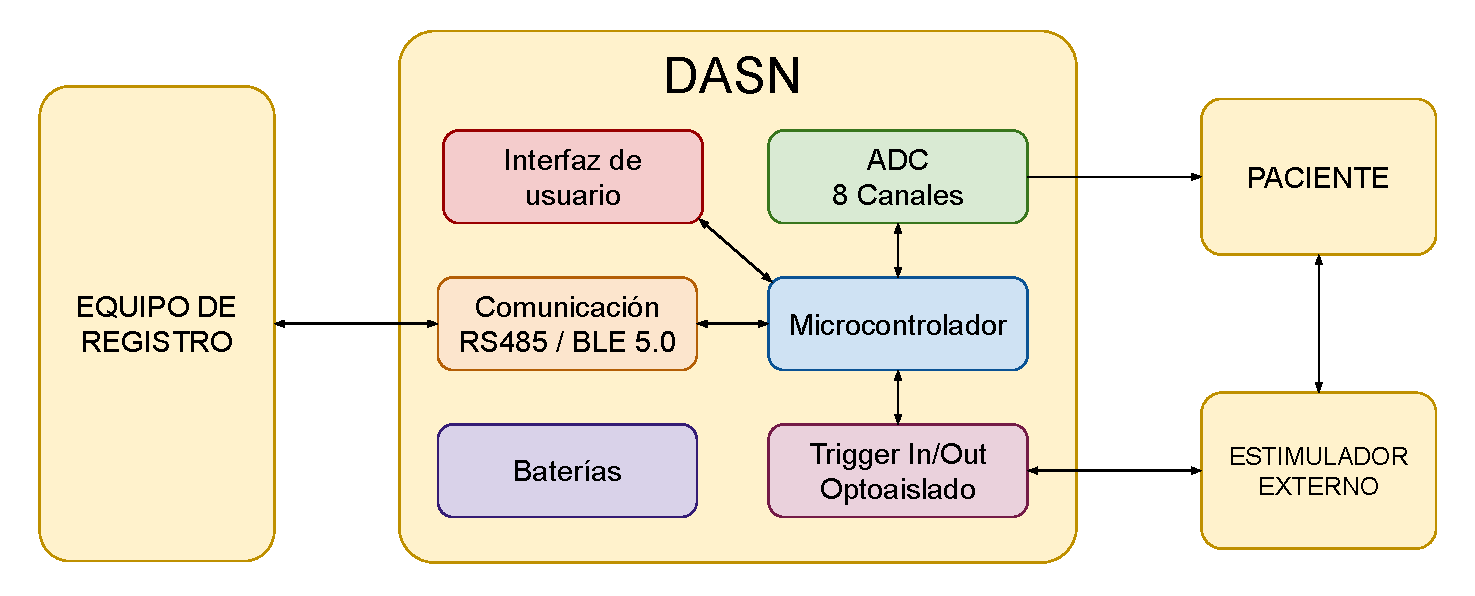
\includegraphics[width=0.94\textwidth]{./Figuras/DiagramaEnBloquesDASN.pdf}
\caption{Diagrama en bloques del sistema}
\label{fig:diagBloquesSistema}
\end{figure}

El DASN tendrá 8 canales de entrada para adquirir las señales neurofisiológicas del paciente y las transmitirá al equipo de registro de manera inalámbrica a través de una comunicación BLE 5.0, o cableada a través de una comunicación RS485. Las señales adquiridas se podrán sincronizar con un estimulador externo, pudiendo funcionar el estimulador como master o slave. La interfaz de usuario solo dará indicaciones de encendido, apagado y estado de funcionamiento, ya que las señales adquiridas se visualizarán en el monitor del equipo de registro. El DASN se alimentará a baterías.

\section{2. Identificación y análisis de los interesados}
\label{sec:interesados}

\begin{table}[ht]
%\caption{Identificación de los interesados}
%\label{tab:interesados}
\begin{tabularx}{\linewidth}{@{}|l|X|X|l|@{}}
\hline
\rowcolor[HTML]{C0C0C0} 
Rol           & Nombre y Apellido & Organización 	& Puesto 	\\ \hline
%Auspiciante   & -		          &\pertesupname  	& -       	\\ \hline
Cliente       & \clientename      &\empclientename	& Director del proyecto     	\\ \hline
%Impulsor      &                   &              	&        	\\ \hline
Responsable   & \authorname       & FIUBA        	& Alumno 	\\ \hline
%Colaboradores &                   &              	&        	\\ \hline
%Orientador    & \supname	      & \pertesupname   & Director trabajo final \\ \hline
Orientador    & \cosupname	      & \pertecosupname   & Codirector trabajo final \\ \hline
%Equipo        & \authorname 	  & FIUBA         	& Alumno  	\\ \hline
%Opositores    &                   &              	&        	\\ \hline
%Usuario final &                   &              	&        	\\ \hline
\end{tabularx}
\end{table}


\section{3. Propósito del proyecto}
\label{sec:proposito}

El propósito de este proyecto es poner en práctica todos los conocimientos adquiridos durante la carrera de especialización, colaborar con el proyecto ''C2-ING-066 Herramientas de uso comunitario para el desarrollo de la industria de Tecnología Neurofisiológica", y a su vez, completar los requisitos de aprobación de la CESE.

\section{4. Alcance del proyecto}
\label{sec:alcance}

El presente proyecto incluye:
\begin{itemize}
	\item Diseño del firmware embebido del DASN.
	\item Diseño del protocolo de comunicación entre DASN y equipo de registro.
	\item Documentación acorde a ISO 62304.
	\item Software de prueba para simular un equipo de registro y probar el DASN.
\end{itemize}

El presente proyecto no incluye:
\begin{itemize}
	\item Diseño de hardware.
	\item Filtrado digital de las señales adquiridas
\end{itemize}


\section{5. Supuestos del proyecto}
\label{sec:supuestos}

Para el desarrollo del presente proyecto se supone que:
\begin{itemize}
	\item El cliente proveerá del hardware necesario para el desarrollo del firmware.
	\item El protocolo de comunicación entre el DASN y el equipo de registro es de libre diseño.
	\item El DASN y el equipo de registro estarán siempre cerca por lo que no hay requisitos de alcance en la comunicación inalámbrica.
	\item El hardware no cambiará durante el desarrollo del proyecto.
\end{itemize}

\section{6. Requerimientos}
\label{sec:requerimientos}

\begin{enumerate}
	\item \textbf{Requerimientos de interfaces externas}
		\begin{enumerate}
			\item El software deberá comunicarse con el equipo de registro utilizando una interfaz BLE 5.0.
			\item El software deberá comunicarse con el equipo de registro utilizando una interfaz RS485. 
			\item El software deberá indicar mediante el led1 que está transmitiendo las señales adquiridas de forma inalámbrica o cableada. 
			\item El software deberá indicar mediante el led2 si está encendido o apagado. También deberá indicar con el mismo led2 si entra en el modo pairing BLE.
			\item El software deberá manejar una salida para sincronizar la adquisición con un estimulador externo (dispositivo externo como slave). La salida deberá poder configurarse entre normal bajo y normal alto. El pulso deberá poder configurarse entre 5 anchos de pulso diferentes (0,1 ms; 0,5 ms; 1 ms; 5 ms; 10 ms). 
			\item El software deberá manejar una entrada para sincronizar la adquisición con un estimulador externo (dispositivo externo como master). La detección deberá ser por flanco y se deberá poder configurar si el flanco es de subida o de bajada.
			\item El software deberá manejar el pulsador que servirá para encender el dispositivo y para realizar el pairing BLE.
			\item El software deberá generar la señal de impedancia para los canales de potenciales evocados.
			\item El software deberá medir el estado de las baterías con el ADC interno del MCU.
		\end{enumerate}
	\item \textbf{Requerimientos funcionales}
		\begin{enumerate}
			\item El software deberá configurar la frecuencia de muestreo de la señal adquirida entre 7 diferentes valores ( el ADC de ''EEG-FrontEnd\_v1.x.0.SchDoc” ofrece 65 Hz, 131 Hz, 262 Hz, 524 Hz, 1048 Hz, 2096 Hz y 4193 Hz).
			\item El software deberá poder adquirir de 1 a 8 canales simultáneos.
			\item Mediante comandos recibidos por BLE 5.0 o RS485 el software deberá poder iniciar y parar la adquisición.
			\item El software deberá configurar la ganancia de amplificación de cada canal entre 7 diferentes valores ( el ADC de ''EEG-FrontEnd\_v1.x.0.SchDoc” ofrece 1, 2, 4, 6, 8, 12 y 24).
			\item El software deberá configurar el ADC para usar una tipología de entrada diferencial o referencial.
			\item El software deberá medir la impedancia de los electrodos con una señal de medición de impedancia cuya frecuencia deberá ser de 7,8 Hz o 31,2 Hz.
			\item El software deberá seleccionar a qué electrodos le inyecta la señal de medición de impedancia.
			\item El software deberá seleccionar para cada electrodo si usa la señal de impedancia generada por el ADC o la generada por el MCU.
			\item El software deberá enviar la siguiente información de autodiagnóstico: temperatura del ADC, valor de las tensiones del ADC y frecuencia del clock del ADC.
			\item El software deberá prender y apagar el equipo con una pulsación corta del botón, pulsación menor a 1 segundo.
			\item El software deberá entrar en el modo de apareo de la comunicación BLE con una pulsación larga del botón, pulsación mayor a 4 segundos.
			\item Luego de 1 minuto de inactividad, el software deberá entrar a un modo de bajo consumo de energía. Para esto deberá apagar el ADC, el transceiver RS485 y la alimentación de todos los periféricos externos al MCU.
			\item El software deberá manejar una comunicación RS485 hasta 3 MBd.
			\item El software deberá poder recibir comandos mientras está transmitiendo las señales adquiridas.

		\end{enumerate}
	\item \textbf{Requerimientos de documentación}
		\begin{enumerate}
			\item La documentación debe cumplir los requisitos de la norma ISO 62304.
			\item Toda la documentación del proyecto se almacenará bajo un sistema de control de versiones GIT.
			\item Toda la documentación del código se realizará utilizando la herramienta Doxygen.
			\item Se deberá realizar un informe de avance del proyecto en el séptimo mes de trabajo
			\item Se deberá realizar la memoria técnica del trabajo final con la plantilla elaborada por la cátedra de gestión de proyecto.
		\end{enumerate}
%	\item \textbf{Requerimientos futuros}
%		\begin{enumerate}	
%			\item En el futuro se prevé diseñar un hardware con hasta 32 canales de adquisición.
			
%		\end{enumerate}
\end{enumerate}

\section{7. Historias de usuarios (\textit{Product backlog})}
\label{sec:backlog}

Criterio para ponderar los \textit{story points}: 

Se deben evaluar los siguientes aspectos de cada historia de usuario con una escala de 1 a 3, donde 1 es la calificación más baja y 3 la más alta:
\begin{itemize}
	\item \textbf{Dificultad} (cantidad de trabajo a realizar).
	\item \textbf{Complejidad} (nivel de sofisticación del trabajo).
	\item \textbf{Incertidumbre} (nivel de riesgo que involucra realizar la tarea).
\end{itemize}	

Finalmente se determina el \textit{story point} realizando la siguiente operación:

\textbf{\textit{Story points}} = Dificultad x Complejidad x Incertidumbre


	\begin{enumerate}
		\item ''Como usuario quiero seleccionar la frecuencia de muestreo y ganancia de cada canal para poder hacer distintos tipos de estudios neurológicos."
		\begin{itemize}
			\item \textbf{Dificultad:} 1
			\item \textbf{Complejidad:} 2
			\item \textbf{Incertidumbre:} 1
		\end{itemize}	
	\textbf{\textit{Story points}} = 2

		\item ''Como usuario quiero que el equipo sea inalámbrico para que el paciente se mueva libremente"
		\begin{itemize}
			\item \textbf{Dificultad:} 2
			\item \textbf{Complejidad:} 3
			\item \textbf{Incertidumbre:} 3
		\end{itemize}	
	\textbf{\textit{Story points}} = 18

		\item ''Como usuario quiero medir la impedancia de los electrodos para poder comprobar su correcta colocación."
		\begin{itemize}
			\item \textbf{Dificultad:} 2
			\item \textbf{Complejidad:} 2
			\item \textbf{Incertidumbre:} 1
		\end{itemize}	
	\textbf{\textit{Story points}} = 4

		\item ''Como usuario quiero sincronizar el equipo con un estimulador externo para hacer estudios de potenciales evocados."
		\begin{itemize}
			\item \textbf{Dificultad:} 2
			\item \textbf{Complejidad:} 2
			\item \textbf{Incertidumbre:} 2
		\end{itemize}	
	\textbf{\textit{Story points}} = 8

		\item ''Como usuario quiero ver el estado de las baterías para saber la autonomía del equipo."
		\begin{itemize}
			\item \textbf{Dificultad:} 2
			\item \textbf{Complejidad:} 2
			\item \textbf{Incertidumbre:} 2
		\end{itemize}	
	\textbf{\textit{Story points}} = 8
	\end{enumerate}

%\begin{consigna}{red}
%Descripción: En esta sección se deben incluir las historias de usuarios y su ponderación (\textit{history points}). Recordar que las historias de usuarios son descripciones cortas y simples de una característica contada desde la perspectiva de la persona que desea la nueva capacidad, generalmente un usuario o cliente del sistema. La ponderación es un número entero que representa el tamaño de la historia comparada con otras historias de similar tipo.
%
%El formato propuesto es: "como [rol] quiero [tal cosa] para [tal otra cosa]."
%
%Se debe indicar explícitamente el criterio para calcular los \textit{story points} de cada historia
%\end{consigna}

\section{8. Entregables principales del proyecto}
\label{sec:entregables}

Los entregables del proyecto son:

\begin{itemize}
	\item Código fuente del firmware.
	\item Código fuente del Software de prueba.
	\item Documentación acorde a ISO 62304.
	\item Informe final
\end{itemize}

%
%\begin{consigna}{red}
%
%Los entregables del proyecto son (ejemplo):
%
%\begin{itemize}
%	\item Manual de uso
%	\item Diagrama de circuitos esquemáticos
%	\item Código fuente del firmware
%	\item Diagrama de instalación
%	\item Informe final
%	\item etc...
%\end{itemize}
%
%\end{consigna}

\section{9. Desglose del trabajo en tareas}
\label{sec:wbs}

En cada grupo de tareas se indica el subtotal de horas correspondiente al mismo.

\begin{enumerate}
\item \textbf{Planificación y documentación (100 hs)}
	\begin{enumerate}
	\item Planificación del proyecto (20 hs)
	\item Especificación de requisitos de software (20 hs)
	\item Investigación Norma ISO 62304 (30 hs)
	\item Análisis de riesgo (30 hs)
	\end{enumerate}
\item \textbf{Diseño e implementación del firmware (270 hs)}
	\begin{enumerate}
	\item Preparación del entorno de desarrollo (20 hs)
	\item Diseño de la arquitectura del firmware  (30 hs)
	\item Investigación sobre tecnología BLE (20 hs)	
	\item Diseño del protocolo de comunicación (30 hs)
	\item Desarrollo del módulo comunicación BLE (40 hs)
	\item Desarrollo del módulo comunicación RS485 (20 hs)
	\item Desarrollo del módulo ADC (30 hs)
	\item Desarrollo del módulo manejo estimulador externo (20 hs)
	\item Desarrollo del módulo interfaz de usuario (10 hs)
	\item Pruebas de integración (30 hs)
	\item Pruebas de verificación (20 hs)
	\end{enumerate}
\item \textbf{Diseño e implementación software de prueba (150 hs)}
	\begin{enumerate}
	\item Preparación del entorno de desarrollo (20 hs)
	\item Diseño de la arquitectura (20 hs)
	\item Desarrollo de drivers (40 hs)
	\item Desarrollo de Interfaz gráfica (30 hs)
	\item Pruebas de integración (20 hs)
	\item Pruebas de verificación (20 hs)
	\end{enumerate}
\item \textbf{Cierre del proyecto (110 hs)}
	\begin{enumerate}
	\item Pruebas de validación (40 hs)
	\item Informes de avance del proyecto (10 hs)
	\item Presentaciones al cliente (10 hs)
	\item Memoria descriptiva final del proyecto  (40 hs)
	\item Presentación final del proyecto (10 hs)
	\end{enumerate}
\end{enumerate}

\textbf{Cantidad total de horas: (630 hs)}

\newpage
\section{10. Diagrama de Activity On Node}
\label{sec:AoN}



\begin{figure}[htpb]
\centering 
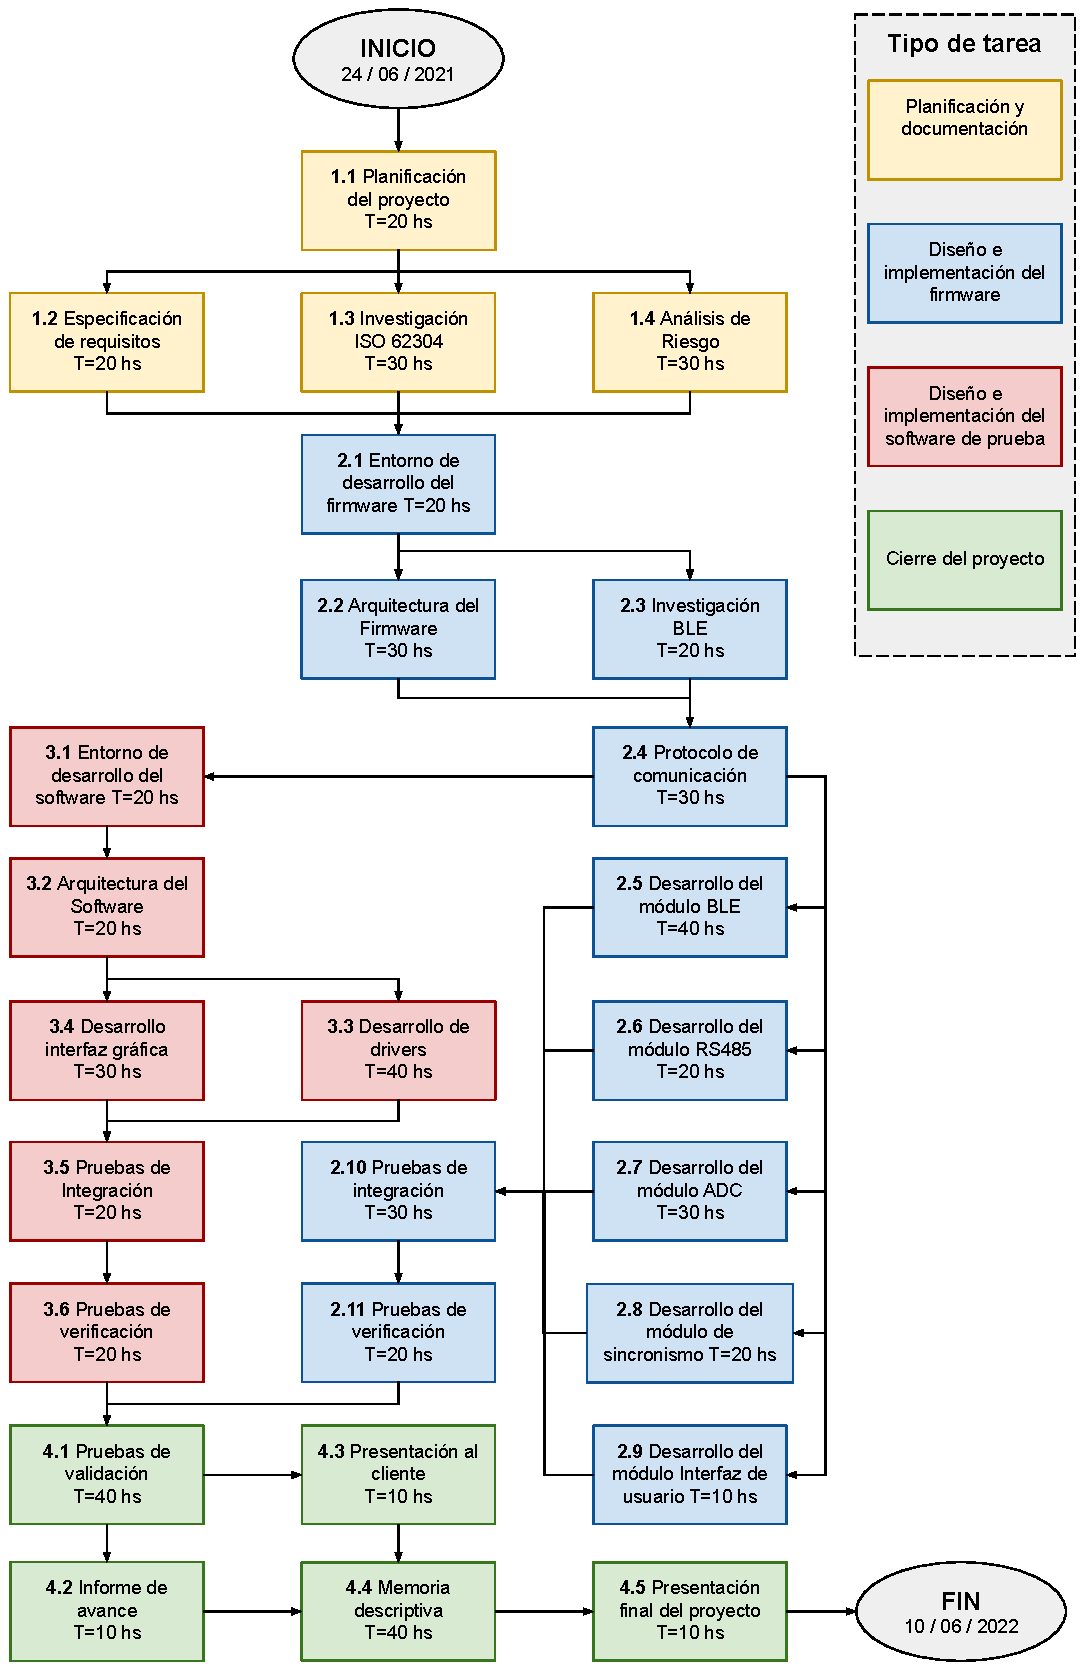
\includegraphics[width=0.75\textwidth]{./Figuras/DASNActivityonNode.pdf}
\caption{Diagrama de \textit{Activity on Node}}
\label{fig:AoN}
\end{figure}

%\begin{landscape}

\section{11. Diagrama de Gantt}
\label{sec:gantt}

\begin{figure}[htpb]
\centering 
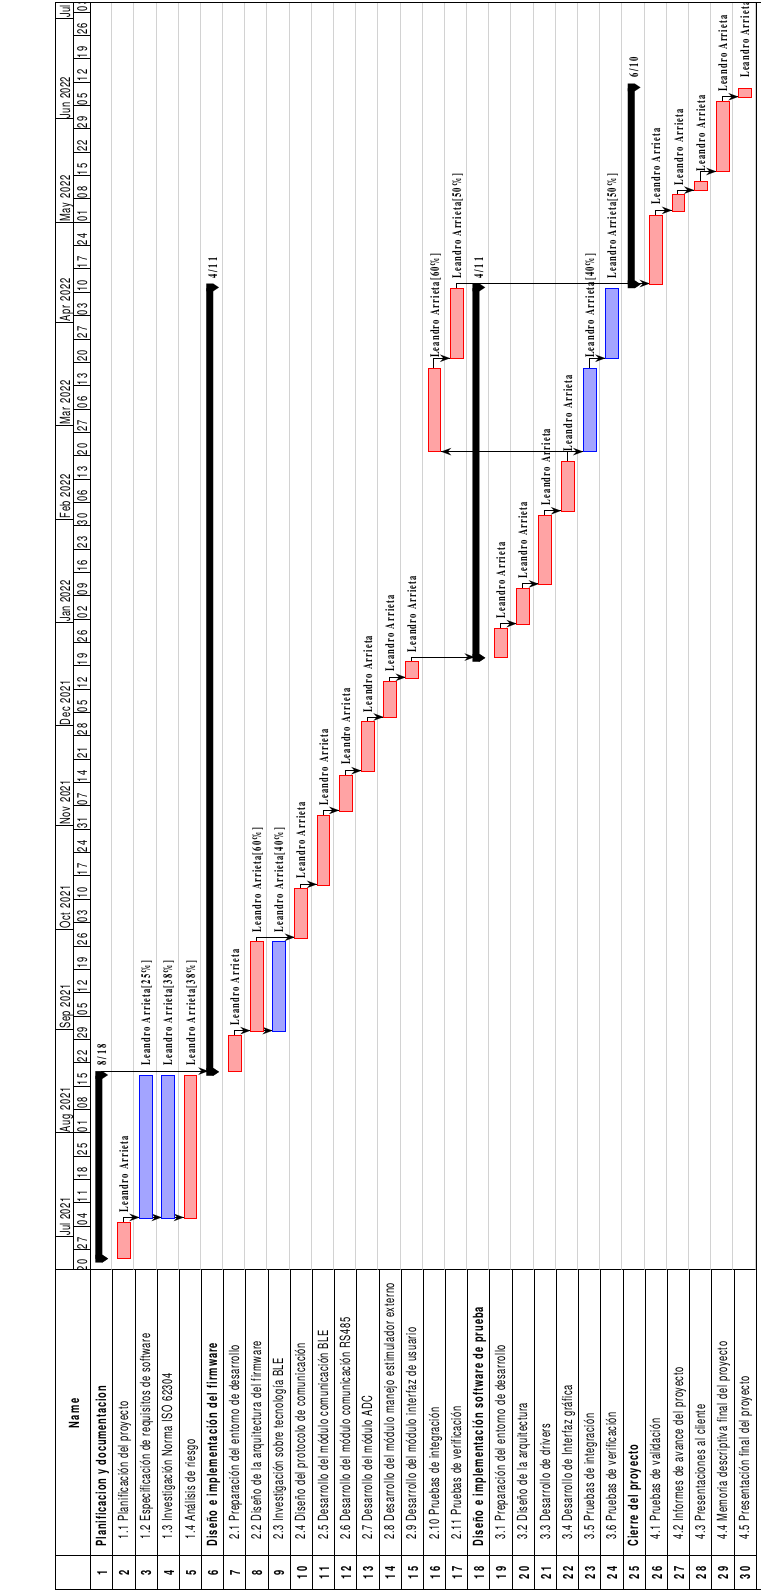
\includegraphics[height=.96\textheight]{./Figuras/DASNGantt.png}
\caption{Diagrama de Gantt}
\label{fig:diagGantt}
\end{figure}

%\end{landscape}


\section{12. Presupuesto detallado del proyecto}
\label{sec:presupuesto}

\begin{table}[htpb]
\centering
\begin{tabularx}{\linewidth}{@{}|X|c|r|r|@{}}
\hline
\rowcolor[HTML]{C0C0C0} 
\multicolumn{4}{|c|}{\cellcolor[HTML]{C0C0C0}COSTOS DIRECTOS} \\ \hline
\rowcolor[HTML]{C0C0C0} 
 Descripción & Cantidad & Valor unitario & Valor total \\ \hline

 Mano de obra & 630 & u\$s 10,00 & u\$s 6300,00 \\ \hline
 Módulo desarrollo LAUNCHXL-CC2640R2 & 2 & u\$s 34,80 & u\$s 69,60 \\ \hline
 Módulo desarrollo ADS1299EEGFE-PDK & 1 & u\$s 238,80 & u\$s 238,80 \\ \hline
\multicolumn{3}{|c|}{SUBTOTAL} & u\$s 6608,40 \\ \hline
\rowcolor[HTML]{C0C0C0} 
\multicolumn{4}{|c|}{\cellcolor[HTML]{C0C0C0}COSTOS INDIRECTOS} \\ \hline
\rowcolor[HTML]{C0C0C0} 
 Descripción & Cantidad & Valor unitario & Valor total \\ \hline

 Costos indirectos, estimados como 20\% de los los costos directos & 1 & u\$s 1321,68  & u\$s 1321,68  \\ \hline

\multicolumn{3}{|c|}{SUBTOTAL} & u\$s 1321,68 \\ \hline
\rowcolor[HTML]{C0C0C0}
\multicolumn{3}{|c|}{TOTAL} & u\$s 7930,08   \\ \hline
\end{tabularx}%
\end{table}


\section{13. Gestión de riesgos}
\label{sec:riesgos}

%\begin{consigna}{red}
%a) Identificación de los riesgos (al menos cinco) y estimación de sus consecuencias:
% 
%Riesgo 1: detallar el riesgo (riesgo es algo que si ocurre altera los planes previstos de forma negativa)
%\begin{itemize}
%	\item Severidad (S): mientras más severo, más alto es el número (usar números del 1 al 10).\\
%	Justificar el motivo por el cual se asigna determinado número de severidad (S).
%	\item Probabilidad de ocurrencia (O): mientras más probable, más alto es el número (usar del 1 al 10).\\
%	Justificar el motivo por el cual se asigna determinado número de (O). 
%\end{itemize}   
%
%Riesgo 2:
%\begin{itemize}
%	\item Severidad (S): 
%	\item Ocurrencia (O):
%\end{itemize}
%
%Riesgo 3:
%\begin{itemize}
%	\item Severidad (S): 
%	\item Ocurrencia (O):
%\end{itemize}
%
%
%b) Tabla de gestión de riesgos:      (El RPN se calcula como RPN=SxO)
%
%\begin{table}[htpb]
%\centering
%\begin{tabularx}{\linewidth}{@{}|X|c|c|c|c|c|c|@{}}
%\hline
%\rowcolor[HTML]{C0C0C0} 
%Riesgo & S & O & RPN & S* & O* & RPN* \\ \hline
%       &   &   &     &    &    &      \\ \hline
%       &   &   &     &    &    &      \\ \hline
%       &   &   &     &    &    &      \\ \hline
%       &   &   &     &    &    &      \\ \hline
%       &   &   &     &    &    &      \\ \hline
%\end{tabularx}%
%\end{table}
%
%Criterio adoptado: 
%Se tomarán medidas de mitigación en los riesgos cuyos números de RPN sean mayores a...
%
%Nota: los valores marcados con (*) en la tabla corresponden luego de haber aplicado la mitigación.
%
%c) Plan de mitigación de los riesgos que originalmente excedían el RPN máximo establecido:
% 
%Riesgo 1: plan de mitigación (si por el RPN fuera necesario elaborar un plan de mitigación).
%  Nueva asignación de S y O, con su respectiva justificación:
%  - Severidad (S): mientras más severo, más alto es el número (usar números del 1 al 10).
%          Justificar el motivo por el cual se asigna determinado número de severidad (S).
%  - Probabilidad de ocurrencia (O): mientras más probable, más alto es el número (usar del 1 al 10).
%          Justificar el motivo por el cual se asigna determinado número de (O).
%
%Riesgo 2: plan de mitigación (si por el RPN fuera necesario elaborar un plan de mitigación).
% 
%Riesgo 3: plan de mitigación (si por el RPN fuera necesario elaborar un plan de mitigación).
%
%\end{consigna}


\section{14. Gestión de la calidad}
\label{sec:calidad}

%\begin{consigna}{red}
%Para cada uno de los requerimientos del proyecto indique:
%\begin{itemize} 
%\item Req \#1: copiar acá el requerimiento.
%
%\begin{itemize}
%	\item Verificación para confirmar si se cumplió con lo requerido antes de mostrar el sistema al cliente. Detallar 
%	\item Validación con el cliente para confirmar que está de acuerdo en que se cumplió con lo requerido. Detallar  
%\end{itemize}
%
%\end{itemize}
%
%Tener en cuenta que en este contexto se pueden mencionar simulaciones, cálculos, revisión de hojas de datos, consulta con expertos, mediciones, etc.  Las acciones de verificación suelen considerar al entregable como ``caja blanca'', es decir se conoce en profundidad su funcionamiento interno.  En cambio, las acciones de validación suelen considerar al entregable como ``caja negra'', es decir, que no se conocen los detalles de su funcionamiento interno.
%
%\end{consigna}

\section{15. Procesos de cierre}    
\label{sec:cierre}

%\begin{consigna}{red}
%Establecer las pautas de trabajo para realizar una reunión final de evaluación del proyecto, tal que contemple las siguientes actividades:
%
%\begin{itemize}
%	\item Pautas de trabajo que se seguirán para analizar si se respetó el Plan de Proyecto original:
%	 - Indicar quién se ocupará de hacer esto y cuál será el procedimiento a aplicar. 
%	\item Identificación de las técnicas y procedimientos útiles e inútiles que se emplearon, y los problemas que surgieron y cómo se solucionaron:
%	 - Indicar quién se ocupará de hacer esto y cuál será el procedimiento para dejar registro.
%	\item Indicar quién organizará el acto de agradecimiento a todos los interesados, y en especial al equipo de trabajo y colaboradores:
%	  - Indicar esto y quién financiará los gastos correspondientes.
%\end{itemize}
%
%\end{consigna}


\end{document}
